\begin{recipe}[source=\url{https://old.reddit.com/r/veganrecipes/comments/9119so/onepot_vegan_tater_tot_casserole/}]{Tater Tot Casserole}
	\index{One Pot}\index{Vegan}\index{Casserole}\index{Cast Iron}
	\begin{figure}
		\centering
		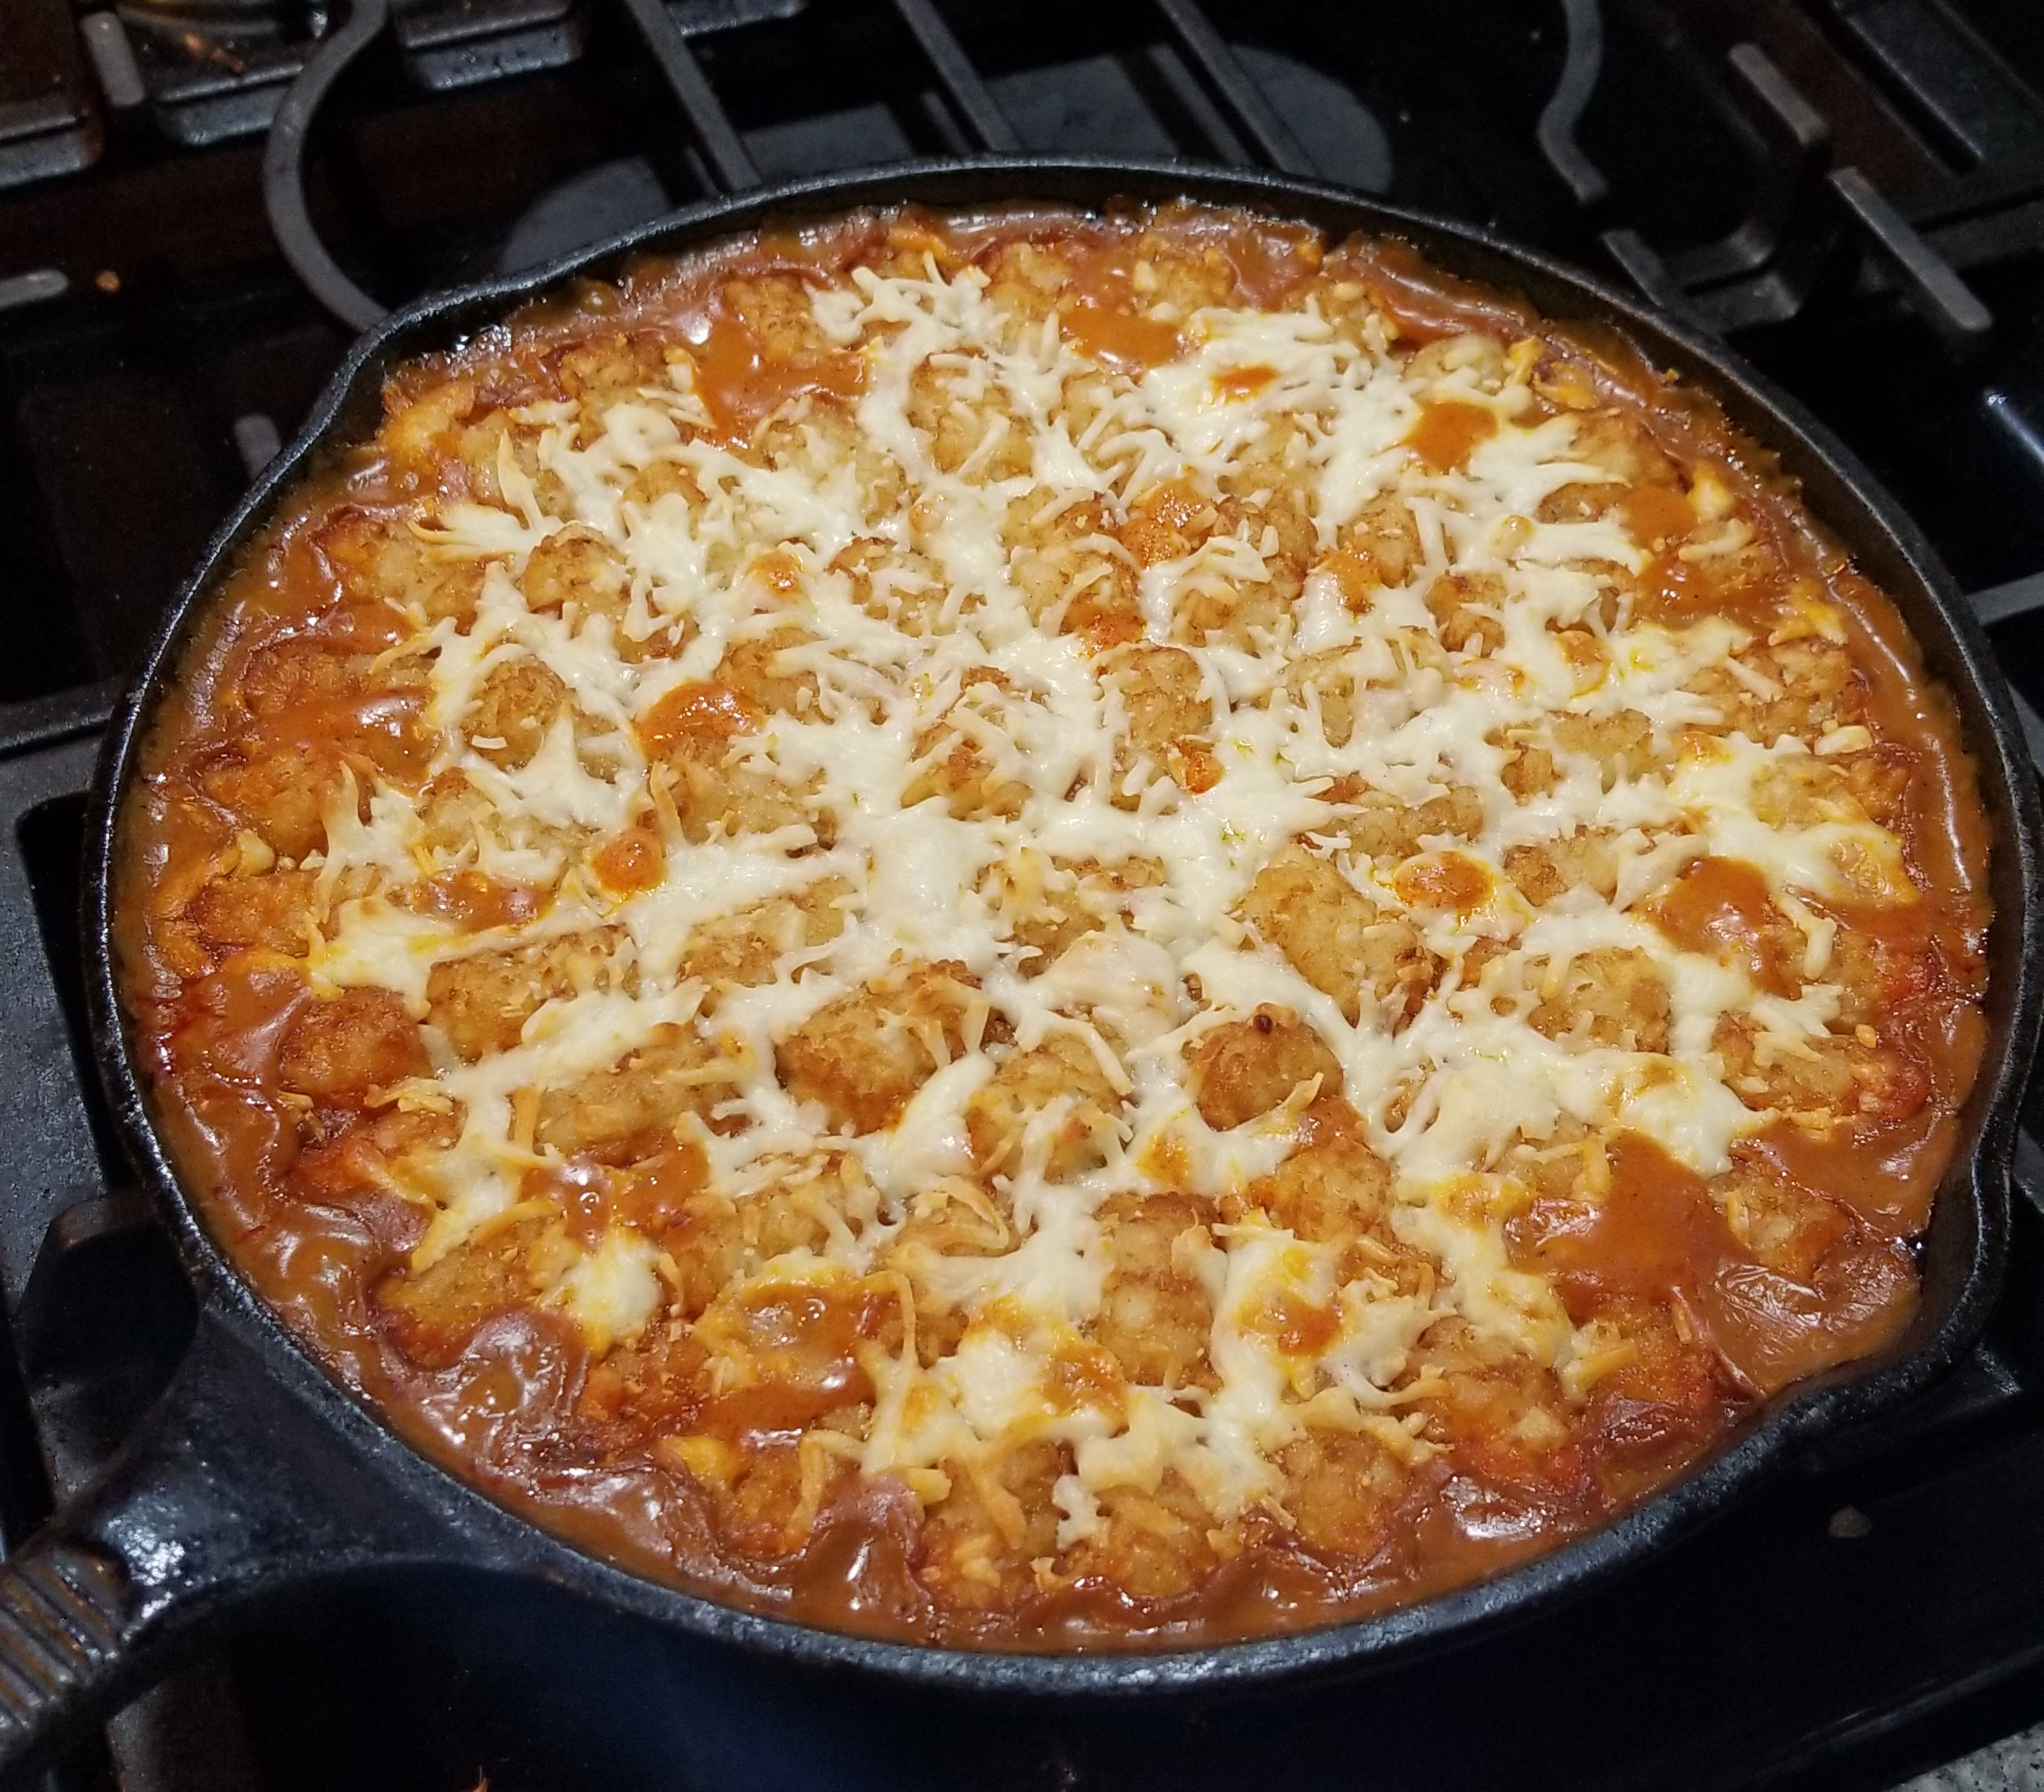
\includegraphics[width=.5\textwidth]{FoodPictures/tatertotcasserole.png}
	\end{figure}
\ingredients[13]{%
	\unit[\nicefrac{1}{2}]{large}& onion \\
	\unit[3]{cloves} & garlic \\
	\unit[6]{patties} & veggie sausage \\
	\unit[1]{can} & cream of mushroom soup \\
	\unit[16]{oz} & frozen veggies \\
	\unit[1]{tsp} & thyme \\
	\unit[1]{tsp} & paprika \\
	\unit[1]{tsp} & chili powder \\
	\unit[1]{tbsp} & flour \\
	\unit[1]{cups} & oat milk \\
	\unit[4]{cups} & tater tots \\
	\unit[1]{cup} & cheese(optional)\\
}
\preparation{%
	\step Preheat the oven to 350 \faren
	\step Heat about a tablespoon of oil in a 12-inch cast iron skillet on medium heat.
	\step Add the onions, cook for 2-3 minutes. Then add the garlic. Continue cooking until the onions are soft and starting to brown.
	\step Add the sausage patties (or other sausage) and stir for a couple of minutes until it starts to brown.
	\step Add the frozen veggies of your choice, mix, and let them cook for another 2-3 minutes.
	\step Add the cream of mushroom soup and mix well to combine.
	\step Add the spices, salt and pepper; thoroughly combine.
	\step Add 1 cup of oat milk and the flour, stir to combine. Then bring to a boil.
	\step Turn off the heat. Then layer the top of the mixture with frozen tater tots.
	\step Place into the oven and bake for 55 minutes.
	\step Remove from the oven and let sit for 5 minutes to cool.
}
\end{recipe}
